\documentclass{article}
\usepackage{pgfplots}
\pgfplotsset{ticks=none}
\begin{document}
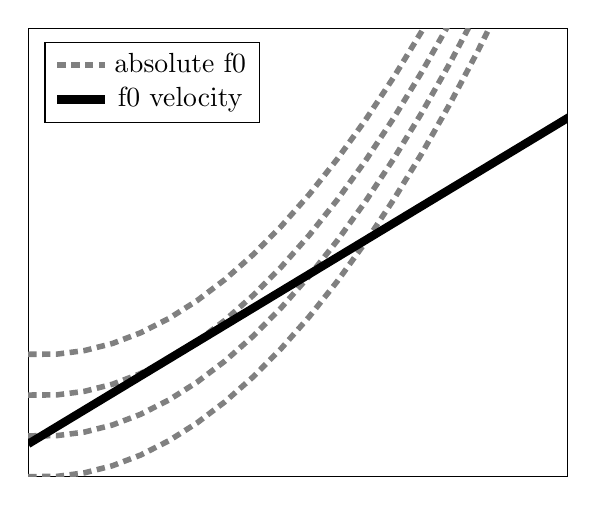
\begin{tikzpicture}
\begin{axis}[no markers, legend pos=north west, domain=0:5, ymin=-5,
  ymax=50, xmin=0, xmax=4, legend entries={absolute f0,,,,f0 velocity}]
\addplot [line width=2pt, densely dashed, black!50] {5*x^2-x-5};
\addplot [line width=2pt, densely dashed, black!50] {5*x^2-x};
\addplot [line width=2pt, densely dashed, black!50] {5*x^2-x+5};
\addplot [line width=2pt, densely dashed, black!50] {5*x^2-x+10};
\addplot [line width=3pt, black] {10*x-1};
%\addplot [black] {((x+0.01)^3-(x)^3)/0.01};
\end{axis}
\end{tikzpicture}

\end{document}